\section{Servidor}


\subsection{Arquitectura}

O servidor é composto vários brokers (idênticos) e uma base de dados. Os brokers são instâncias de uma aplicação desenvolvida em Ruby e a base de dados é PostgreSQL.

\subsection{Mensagens}

As mensagens que o servidor reconhecem são no seguinte formato:

[[instructions], message]

Pode resumir-se que é um array que contém uma lista de instruções na posição zero e uma mensagem na posição um. Existem os seguintes tipos de mensagens:

\begin{enumerate}
\item
\texttt{[[``subscribe''], ``channel'']}

Quando a primeira instrução é ``subscribe'' o servidor subscreve o cliente ao canal com o nome que vai no lugar da mensagem.

\item
\texttt{[[``unsubscribe''], ``channel'']}

Quando a primeira instrução é ``unsubscribe'' o servidor remove a descrição do cliente ao canal com o nome que vai no lugar da mensagem.

\item
\texttt{[[``all''], ``message'']}

Quando a primeira instrução é ``all'' a mensagem é enviada a todos os clientes do servidor (clientes de todos os brokers).

\item
\texttt{[[``channel 1'', ``channel 2''], ``message'']}

Quando a primeira instrução nao é ``all'' então todos as instruções são consideradas nomes de canais e a mensagem é distribuída por todos os clientes subscritos ao canal.
\end{enumerate}

\subsection{Ciclo de Vida de um Cliente}

\begin{figure}[H]
\centering
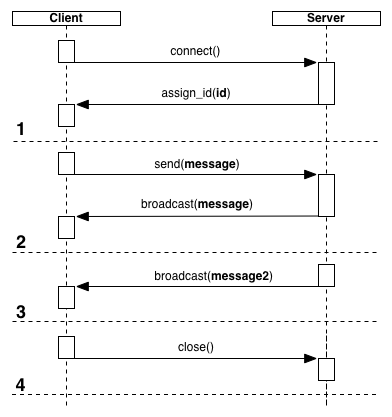
\includegraphics[width=0.65\textwidth]{server_client.png}
\caption{\textit{Ciclo de vida de um cliente.}}
\label{fig:server-client}
\end{figure}

A figura~\ref{fig:server-client} contém um diagrama de sequência que apresenta o básico da interação entre um cliente e o servidor (entenda-se por servidor como um broker do servidor).
Um cliente começa por establecer ligação a um dos brokers do servidor. Assim que a ligação é establecida o broker devolve um identificador único ao cliente. Esta etapa está identificada no bloco um na figura~\ref{fig:server-client}. Depois esta etapa inicial são três os cenários possíveiseservidor

\begin{itemize}
\item
\textbf{O cliente envia uma mensagem}

O cliente envia uma mensagem ao broker (etapa 2 da figura~\ref{fig:server-client}). A mensagem é devolvida ao cliente no processo de broadcast do servidor. 

\item
\textbf{O servidor faz broadcast de uma mensagem}

O servidor envia uma mensagem no processo de broadcast de mensagens de outros clientes (etapa 3 da figura~\ref{fig:server-client}).

\item
\textbf{O cliente termina a ligação}

O cliente termina a ligação com o servidor (etapa 4 da figura~\ref{fig:server-client}).
\end{itemize}
